\documentclass{dsekkallelse}

\usepackage[T1]{fontenc}
\usepackage[utf8]{inputenc}
\usepackage[swedish]{babel}

\setheader{Policy för Ekonomirutiner}{Policydokument}{}

\title{Policy för Ekonomirutiner}
\author{Anna Qvil, Fred Nordell}

\begin{document}

\section{Policy för Ekonomirutiner}

\subsection{1 Bakgrund och Syfte}
D-sektionen är en ideell förening och har inget vinstintresse. Därmed skall ingen funktionär inom D-sektionen behöva betala pengar ur egen ficka för att kunna utföra sitt uppdrag så som uppdraget är beskrivet i reglementet. Ingen funktionär ska tjäna pengar på sektionens verksamhet.
\par Denna policy beskriver D-sektionen syn på ekonomirutiner och attesteringsrätt. Syftet är att ge styrelsen såväl som funktionärer vägledning i frågor gällande kontanthantering, utlägg samt attestering. 

\subsubsection{1.1 Historik}
Policyn är antagen på VTM 2017.  

\subsection{2. Bestämmelser}
Sektionens utskott köper varor och tjänster av varandra till inköpspris.

Projektkommittéer beslutade av styrelsen kan enbart få tillgång till belopp upp till 3000 kr per termin.

\subsubsection{2.1 Avtal}
Firmatecknare äger alltid rätt att besluta om avtal då det innebär ett
positivt nettoresultat samt avtal som följer redan lagd budget. En förutsättning är att avtal
inte går emot D-sektionen eller Teknologkårens styrdokument.
\subsubsection{2.2 Utlägg}
Nedan följer punkter som sektionsmedlemmar ska följa vid utlägg.
\begin{itemize}
\item utläggs- och intäktsräkningar skall skyndsamt lämnas in till Skattmästeriet om ej särskilda skäl finns.
\item utlägg större än 1000 SEK som direkt medverkar till större budgetavsteg och/eller inte direkt kan kopplas till daglig verksamhet ska först godkännas på ett styrelsemöte/sektionsmöte. Styrelsemötet/sektionsmötet äger tolkningsrätt i vad som anses vara daglig verksamhet. 
\end{itemize}

\subsubsection{2.3 Kontanthantering}
Nedan följer punkter som sektionsmedlemmar ska följa vid kontanthantering.
\begin{itemize}
\item kontantbelopp som överstiger 3000 kronor skall och måste räknas av minst två personer.
\end{itemize}

\subsubsection{2.4 Attesteringsrätt}
Nedan följer punkter som sektionsmedlemmar ska följa vid attestering.
\begin{itemize}
\item samtliga utlägg skall signeras av två individer, personen som gjort utlägget och en som godkänner utlägget. Godkännandet ska, om möjligt, utföras av individ från den närmst följande instansen enligt diagram nedan. 
\item utlägg kan inte godkännas av samma individ som gjort utlägget.
\item en högre instans kan i samtliga fall ersätta en lägre instans signatur om så behövs. En lägre instans kan aldrig godkänna en högre instans utlägg.
\item en individ signerar alltid i egenskap av sin högsta instans.
\end{itemize}
\par Nedan följer hur attesteringsrätt fungerar för mästare, vice skattmästare och firmatecknare. Attestering skall alltid sträva efter att skötas på lägsta möjliga instans. Diagrammet nedan är endast för vägledning, nedanstående punkter beskriver mer exakta bestämmelser. Således har inte godtycklig styrelseledarmot attesteringsrätt för teknikfokusansvarig eller utedishoansvarig även fast diagrammet antyder detta.
\begin{itemize}
\item \textbf{Firmatecknare} äger attesteringsrätt för alla utlägg och kan attesteras av varandra. Firmatecknare kan inte attestera sina egna utlägg. 
\item \textbf{Vice skattmästare} äger attesteringsrätt för alla utlägg gjorda av funktionär. Vice skattmästare kan inte attestera styrelseledamöter, utedischoansvarig eller teknikfokusansvarig. 
\item \textbf{Näringslivsansvarig} äger attesteringsrätt för alla utlägg gjorda för näringslivsutskottet, där även utlägg gjorda av teknikfokusansvarig. 
\item \textbf{Studierådsordförande} äger attesteringsrätt för alla utlägg gjorda för studierådet. 
\item \textbf{Vice ordförande} äger attesteringsrätt för alla utlägg gjorda för trivselrådet. 
\item \textbf{Programmästare} äger attesteringsrätt för alla utlägg gjorda för programmästeriet, där även utedishoansvarig. 
\item \textbf{Propagandamästare} äger attesteringsrätt för alla utlägg gjorda för propagandamästeriet. 
\item \textbf{Sexmästare} äger attesteringsrätt för alla utlägg gjorda för sexmästeriet. 
\item \textbf{Cafémästare} äger attesteringsrätt för alla utlägg gjorda för cafémästeriet.
\item \textbf{Källarmästare} äger attesteringsrätt för alla utlägg gjorda för källarmästeriet. 
\item \textbf{Överphös} äger attesteringsrätt för alla utlägg gjorda för nollningsutskottet. 
\item \textbf{Utedishoansvarig} äger attesteringsrätt för alla utlägg gjorda för utedishot. 
\item \textbf{Teknikfokusansvarig} äger attesteringsrätt för alla utlägg gjorda för teknikfokus. 
\end{itemize}

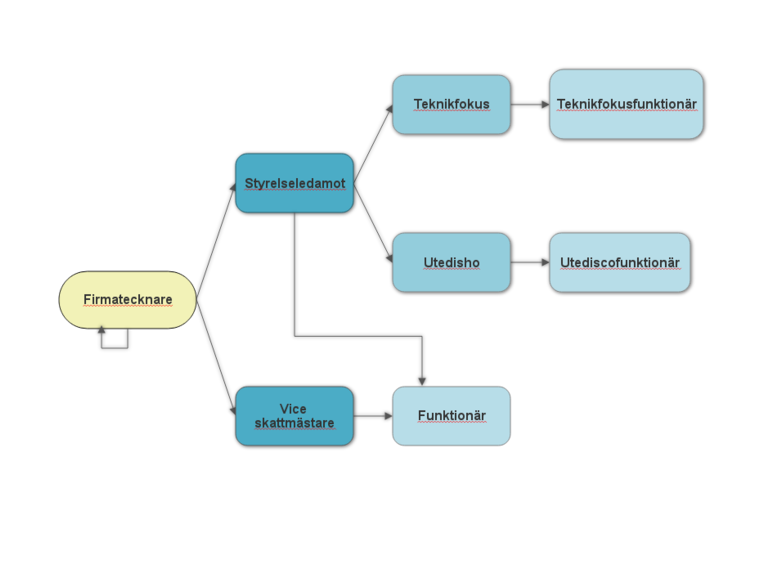
\includegraphics[width=\textwidth]{flow.png}

%\vfill
%\signature{För Styrelsen}{Anna Qvil}{Ordförande, Datatekniksektionen}
%\signature{För Styrelsen}{Fred Nordell}{Skattmästare, Datatekniksektionen}


\end{document}